\pdfminorversion=7
\documentclass[../main.tex]{subfiles}

\begin{document}
\ifx\chapincluded\undefined
  \begin{refsection}[main-bib]
 \fi

 \chapter{Research Contributions}
\label{chap:rcontrib}

The research contributions of this thesis are presented as five articles. The first four (\Cref{chap:cal-paper,chap:pact-paper,chap:wosc-paper,chap:hpca-paper}), and the last (\Cref{chap:eurosys-paper}) is pending review at the time of thesis submission. In this chapter, we summarize the contributions of each paper and contextualize the papers in regard to prior work. The papers that are included in this thesis are:




\section{Contribution overview}

\subsection{Research direction 1: Hardware}
We present our results in two parts where the first partI
(\Cref{subsub:understanding}) covers the
background study, presented in Paper A1 (\Cref{chap:wosc-paper}) and
the second part (\Cref{subsub:btbx}) describes BTB-X, the proposal for a
redesigned BTB proposal covered in Papers
A2, A3 and A4 (\Cref{chap:cal-paper,chap:pact-paper,chap:hpca-paper}).

\subsubsection{Understanding FaaS}
\label{subsub:understanding}
\paragraph{Motivation.} Function-as-a-service (FaaS) computing is a rapidly growing cloud computing model. In FaaS, the unit of computation is a function, normally with a very short execution time. Since a FaaS function is loaded and started when it is needed and shut down when it has finished executing, will co-schedule a large number of functions on the same processors to maximize server utilization. Recent work has reported that this heavily interleaved execution leads to microarchitectural state thrashing causing most of FaaS function execution to occur on a cold microarchitectural state~\cite{shahrad19_archit_implic_funct_servic_comput,lukewarm_serverless}. This work, however, stops short of investigating which specific properties of FaaS execution that causes this poor utilization of microarchitectural state.

\paragraph{Approach.}
To address this gap in the research, we perform an evaluation of FaaS
functions executed on a processor with warm and cold
microarchitectural states respectively. We use a representative suite
of FaaS functions consisting of both real-world and synthetic
workloads. Using synthetic workloads allow us to modify specific
parameters of interest in a targeted way. To measure the impact of
executing the functions on a warm and cold microarchitectural state we
execute the functions in tow modes: back-to-back and interleaved. In
back-to-back execution, the functions are executed repeatedly in a
tight loop. In the interleaved execution case, each invocation of a
function is interleaved with an invocation of a \emph{trhasher}
function that thrashes all existing microarchitectural state. The
thrasher function achieves this by performing two
actions: \begin{inparaenum}[1)]
\item it invokes the x86 WBINVD
  instruction that writes back and invalidates the entire cache
  hierarchy of the processor package~\cite[Chapter 6]{intelmanual} and \item it runs a function that
  executes a long sequence of branches in order to thrash the state of
  the BTB and the branch predictor. \end{inparaenum} We measure
microarchitectural parameters using perf~\cite{perftool} and use the Top-Down
methodology~\cite{yasin14_top_down} for identifying specific
microarchitectural bottlenecks. For both the back-to-back and
interleaved execution we measured both the wall-clock running time of
the functions and key microarchitectural parameters.

To support our findings (presented below) we perform a measurement of
the code footprint of each of the FaaS functions that we use in our
analysis. Doing this using a full microarchitectural simulator is a
slow and tedious process and it is not possible to perform this
analysis statically since the dynamic instruction trace of a program
is only known at runtime.  Therefore, we use a method described
in~\cite{splash2} that use branch-record traces and a cache simulator
to estimate the code footprint of a function. The branch-record traces
show the branches taken by a program. By running the locations of
these branches through a cache simulator, we can measure how big the
cache has to be in order to fit the entire code footprint of a
program. More specifically this is done by changing the size of the
simulator cache until the observed miss-rate reaches zero. When this
is the case, the entire code footprint of the program fit inside the
cache.


\paragraph{Key Results.}
Our results show that two properties of a FaaS function impacts how
sensitive it is to being executed on a cold microarchitectural state:
Its execution time and its code footprint. For example, the shortest
running function that we evaluate (0.25 ms) show a slowdown of
$17\times$ when executed on a processor with a cold microarchitectural
state. The longest running functions are largely unaffected by
microarchitectural state thrashing. This indicates that the warm-up
latency of microarchitectural structures is amortized for the vast
majority of FaaS functions.

Another important observation we make from our experiments, is that
the real-world FaaS functions we evaluate are overwhelmingly front-end
bound. This is in line with similar observations made for general
server
workloads~\cite{ferdman12_clear_cloud,kanev15_profil,ayers19_asmdb}
and for FaaS functions specifically~\cite{lukewarm_serverless}. This
strongly motivates further research aiming to alleviate the front-end
bottleneck with the goal of optimizing the execution of FaaS
functions.

\subsubsection{A storage-efficient BTB organization for servers}
\label{subsub:btbx}

\paragraph{Motivation.}
The front-end bottleneck is a well-known and widely documented problem
affecting processors executing server
workloads~\cite{ailamaki99_dbmss_moder_proces,ferdman12_clear_cloud,kanev15_profil,ayers19_asmdb}. Compared
to other workload classes, server workloads pose particular challenges
for processor frontends due to their very large instruction
footprints. These footprints, quickly overwhelms the capacities of the
instruction cache L1-I) and the Branch Target Buffer (BTB). In order
to handle this problem, computer architects has proposed a large
number of different approaches. L1-I prefetchers are a highly
effective way to alleviate the front-end bottleneck as they help
avoiding the fill-latency that follows an L1-I miss.  As detailed in
\truls{Add reference to relevant background section}, a particularly
effective class of instruction prefetchers are known as Fetch Directed
Instruction Prefetching
(FDIP)~\cite{reinman99_fetch_direc_instr_prefet}. Since FDIP rely on
the BTB to predict the control flow of a program, having a BTB with
sufficient capacity is of crucial importance. By simply scaling the
design of a conventional BTB design, the capacity required for holding
realistic branch working sets of contemporary server workloads quickly
become infeasible. To address this, previous work observed that all
branch targets within a page share the same numbers and only differ in
page offsets. Thus the page number can be deduplicated by only storing
it once in a dedicated table and then replacing its use in a branch
target address with a pointer to that
table~\cite{seznec96_dont_use_page_number_point_it}. \textcite{soundararajan21_pdede}
extends this concept further by observing that several branch page
numbers share a common region number which can be deduplicated
further. The limitation of these approaches is that they introduce a
level of indirection for BTB lookups, adding complexity and increasing
the BTB access latency.


\paragraph{Approach.}

\begin{figure}[ht]
  \centering
  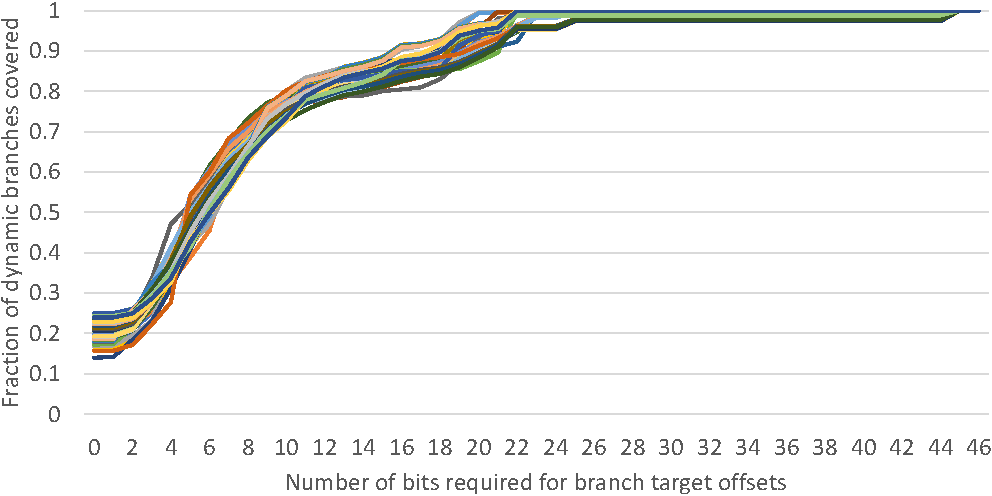
\includegraphics[width=0.8\textwidth]{figures/offset_distribution.pdf}
  \caption{\label{fig:offset-distr} Distribution of branch target offsets in the IPC-1~\cite{ipc1} workload traces}
\end{figure}

To gain a deeper understanding of the characteristics of branch
targets, we performed an analysis of the branch target offsets in a
large number of real-world workload traces released for the first
Instruction Prefetching Championship (IPC-1)~\cite{ipc1}. A branch
target offset is the distance from a branch to its target. From this
analysis, shown in \Cref{fig:offset-distr} we make the observation
that the vast majority of branches have targets very close to their
origin. For example, using just 19 bits we can represent the target
offsets of 90\% of all branches. This is significantly less than the
46 bits\footnote{This is assuming an Arm-64 architecture whre all
  instructions are 4 bytes long. Thus, we save the last two offset
  bits of the full 48-bit virtual address space.} required to store
the full target address.

\begin{figure}[ht]
  \centering
  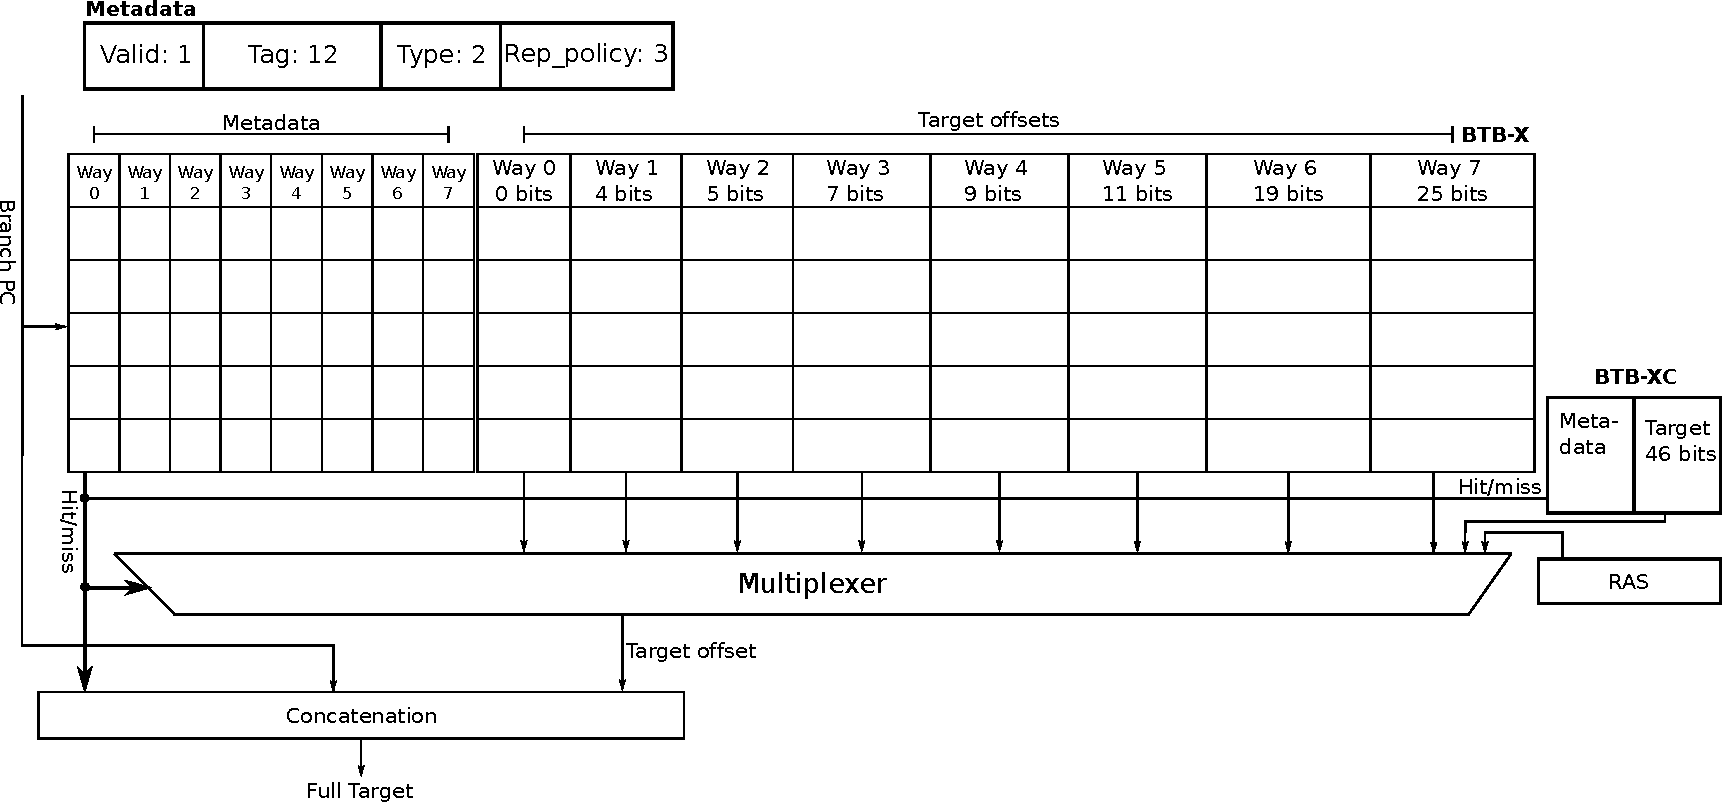
\includegraphics[width=\textwidth]{figures/BTB-X.pdf}
  \caption{\label{fig:btbx-design} The design of BTB-X.}
\end{figure}

Based on this observation we propose BTB-X, a redesigned BTB that uses
differently sized ways matching the distribution of target offset
sizes that we observed. To accommodate branch targets that require the
full address size, we introduce we use conventional BTB called
BTB-XC. When accessing the BTB, BTB-X and BTB-XC are looked up in
parallel. The full design of BTB-X is shown in \Cref{fig:btbx-design}.

We implement and evaluate BTB-X using the Champsim
simulator. Champsim is a trace-based simulator for microarchitectural
studies~\cite{champsim}. For evaluation we use the aforementioned
workload traces released as part of the IPC-1 championship. The traces
were provided by Qualcomm and include both server and client
workloads. For the BTB-X design to be applicable to all workloads, the
branch target offset size distribution that guided its design must be
shown to be widely applicable. To ensure this, we measure the branch
target offset size distributions of the more than 750 traces provided by
Qualcomm as part of the First Championship Value Prediction CVP-1 and
traces from 6 known server applications. These results show nearly
identical branch target offset size distributions.

Finally, we measure the energy requirements and access latencies of
BTB-X, the state-of-the-art BTB design and a conventional BTB using Cacti 7.0~\cite{cacti} at the 22nm technology node.

\paragraph{Key Results.}

Our evaluation show that, BTB-X stores 2.24\texttimes more branches
than a conventional BTB organization. Furthermore, when compared to
the state of the art BTB design PDede, BTB-X stores  and
1.24\texttimes and 1.34\texttimes more branches for storage budgets of
0.9KB and 59KB respectively. This increase in branch storage density
translates to a significant increase in BTB MPKI. 

% \truls{Emphasize how the evaluation methodology using the traces from server workloads applies to FaaS workloads since a) they are fundamentally similar except that FaaS workloads run for a shorter time and b) we and prior work shows that FaaS workloads also have a large code footprint}

\subsection{Research direciton B: Software optimizations for serverless computing}

\paragraph{Motivation.}


\paragraph{Approach.}

\paragraph{Key Results.}


%\subsection{Primary contribution 2: 

\ifx\chapincluded\undefined
  \printbibliography
  \end{refsection}
 \fi
\end{document}


%%% Local Variables:
%%% mode: latex
%%% TeX-master: t
%%% TeX-command-extra-options: "-shell-escape"
%%% End: